\section{Introduction}
\label{sec:introduction}

Reinforcement Learning with Verifiable Rewards (RLVR) has rapidly reshaped the landscape of large language model (LLM) reasoning, driving landmark systems such as OpenAI o1~\citep{openai2024openaio1card} and DeepSeek R1~\citep{Guo_2025}. A dominant narrative attributes the success of these RL approaches, most notably Group Relative Policy Optimization (GRPO)~\citep{schulman2017proximalpolicyoptimizationalgorithms, shao2024deepseekmathpushinglimitsmathematical, yu2025dapoopensourcellmreinforcement}, to their on-policy design, where rollouts are freshly generated and closely aligned with the current policy. This freshness is widely viewed as important for stable credit assignment and iterative self-improvement.

On closer inspection, however, standard GRPO implementations are almost never strictly on-policy. The off-policyness arises from multiple sources. One primary source is data staleness: most RL training frameworks~\citep{sheng2025hybridflow, slime_github, noukhovitch2024asynchronous, zhong2025streamrl, he2025history} use rollouts generated by policies from several updates earlier, resulting in a \emph{near} on-policy regime that trades off rollout freshness for efficiency~\citep{huggingface_openr1_update3}. Throughout this paper, we refer to this commonly used low-staleness, near-on-policy implementation as \emph{standard GRPO}. Another source of off-policyness stems from training–inference mismatch. In practice, rollouts are typically generated using high-throughput inference backends like vLLM~\citep{kwon2023efficientmemorymanagementlarge}, while policy optimization is performed using sharded training engines like FSDP~\citep{zhao2023pytorchfsdpexperiencesscaling}. This introduces numerical discrepancies between rollout generation and optimization. Empirically, however, LLM RL has proven tolerant to such off-policyness when appropriate stabilization techniques are applied~\citep{liu-li-2025-rl-collapse,qi2025defeating}.




Taken together, these observations raise a natural question: \textit{How far can we increase rollout staleness in GRPO without compromising learning stability or reasoning performance?}
% \begin{figure}
% \centering
% 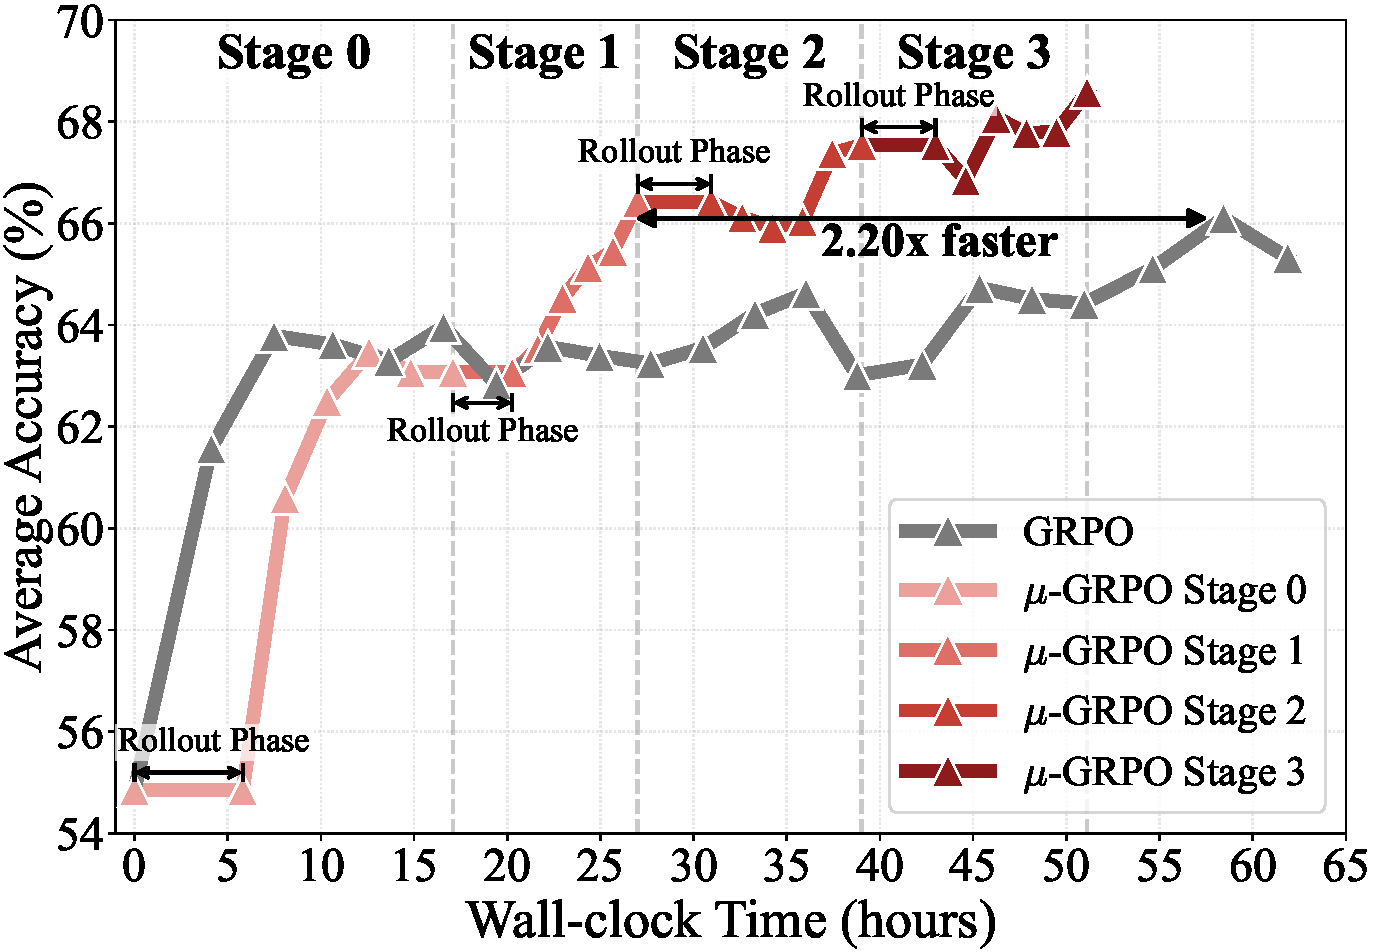
\includegraphics[width=0.47\textwidth]{figures/teaser.pdf}
% \caption{Wall-clock efficiency comparison between on-policy GRPO ($\mu\!=\!4$) and high-staleness $\mu$-GRPO ($\mu\!=\!1024$) over 4096 model updates, evaluated on DeepSeek-7B \citep{shao2024deepseekmathpushinglimitsmathematical}.
% Curves show average accuracy (\%) across five evaluation benchmarks as a function of wall-clock time (hours).
% Stage durations are non-uniform, reflecting changes in the model’s mean response length during training, which affect rollout generation and per-step computation costs and thus result in varying wall-clock times.}
%     \label{fig:teaser}
% \end{figure}


\begin{wrapfigure}{r}{0.6\linewidth}
% \vspace{-pt}
\centering
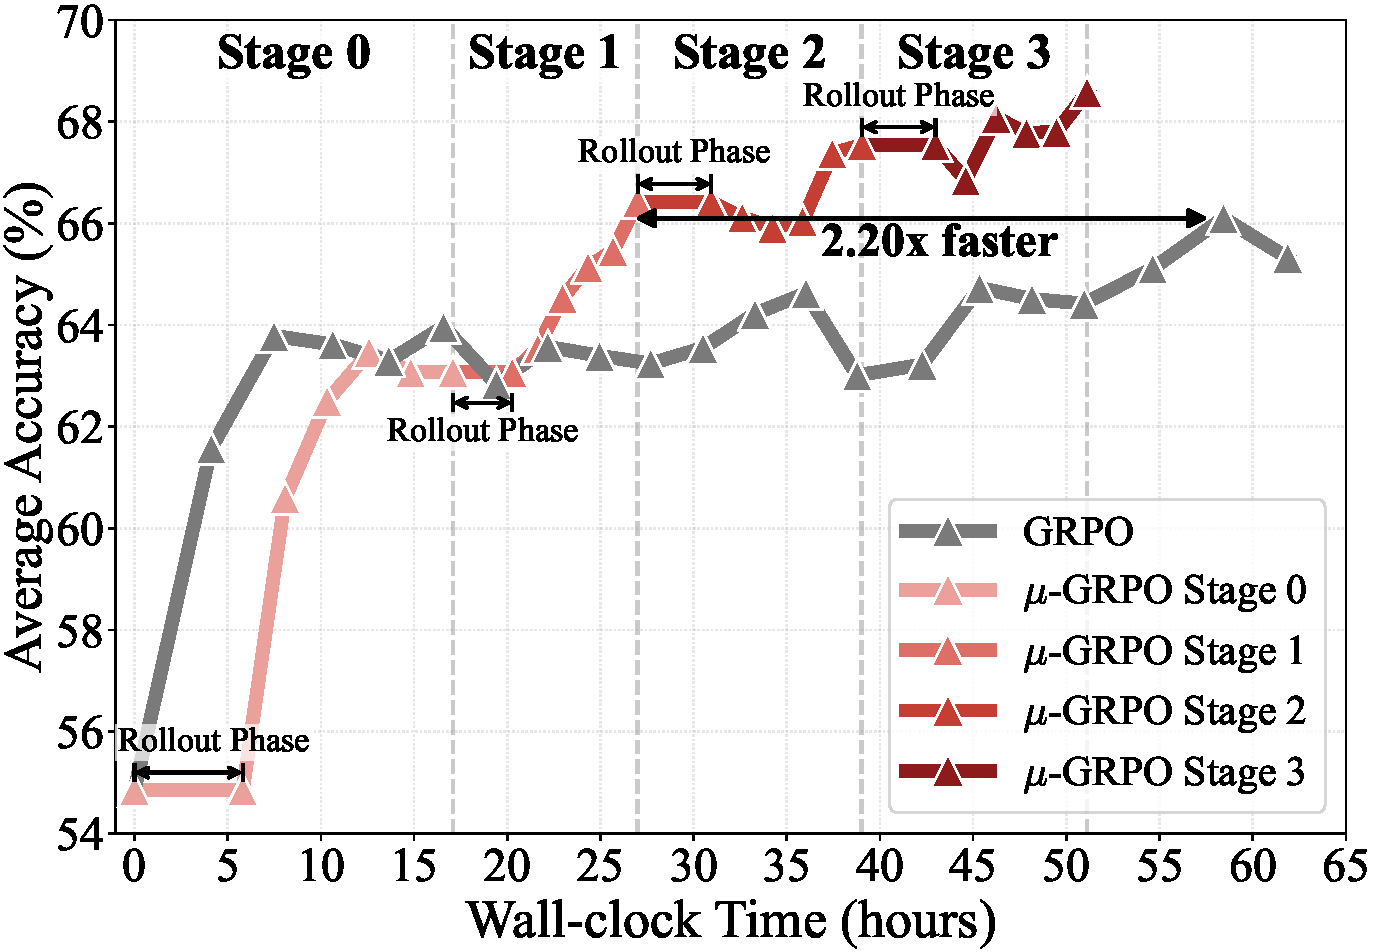
\includegraphics[width=\linewidth]{figures/teaser.pdf}
\caption{
\textbf{Comparing GRPO and \boldmath \ourmethod.}
Average accuracy across five math benchmarks over
wall-clock time. \ourmethod{} uses four large rollout--optimization stages, inducing high rollout
staleness while reducing rollout--training switching overhead. It reaches GRPO's
performance with a 2.2$\times$ wall-clock speedup on DeepSeek-7B~\citep{shao2024deepseekmathpushinglimitsmathematical}.
Both methods are trained for 4096 updates.
}
\label{fig:teaser}
\vspace{-14pt}
\end{wrapfigure}

This question is also central to system efficiency. Standard GRPO implementations repeatedly alternate between rollout generation and policy optimization, requiring many weight synchronizations between inference and training engines. To make such switching practical, systems often keep training state resident during rollout generation, reducing memory available for high-throughput inference\citep{sheng2025hybridflow, slime_github}. Increasing rollout staleness could amortize rollout generation over many more policy updates and thereby reduce these overheads. While prior work has explored limited staleness, these approaches do not push staleness far enough to fully decouple rollout generation from optimization~\cite{zheng2025prosperitycollapsefaroffpolicy,xi2025bapo}.

In this paper, we show that GRPO-style algorithms can tolerate substantially larger rollout staleness than commonly assumed, but only if the failure mode of high-staleness optimization is handled explicitly. Our diagnosis reveals that stale rollouts still contain useful learning signal: relaxing the standard GRPO clipping range can recover strong early learning under large staleness. The resulting instability is more localized than a generic off-policy collapse.  We trace it to negative-advantage trajectories that cross an off-support boundary: after the prefix becomes poorly supported by the current policy, token-level GRPO can still apply substantial updates to later suffix tokens. This prefix-support mismatch explains why token-level clipping alone fails under large staleness.


Motivated by this diagnosis, we propose  \textbf{\boldmath{$\mu$}-GRPO}, a staged GRPO framework for high-staleness training. Instead of frequent small generation–optimization cycles, $\mu$-GRPO operates in a small number of large stages. At the beginning of each stage, $\mu$-GRPO freezes the current policy and generates responses for a large prompt set, rather than for a small rollout batch as in standard GRPO. This forms a static rollout dataset that is consumed over many subsequent policy updates using stored behavior log-probabilities as anchors, resulting in extremely high rollout staleness. To stabilize optimization under extreme staleness, \ourmethod{} combines relaxed clipping with negative-advantage veto, which filters destabilizing post-boundary negative-advantage tokens while preserving useful stale-rollout gradients.


 Empirically, $\mu$-GRPO converts GRPO's staleness tolerance into substantial wall-clock speedups. As illustrated in \cref{fig:teaser}, $\mu$-GRPO completes training in a few stages (e.g., four) and exceeds the performance of the standard GRPO while achieving a 2.2$\times$ wall-clock speedup on DeepSeek-7B\footnote{
DeepSeek-7B denotes the Qwen2.5-Math-7B model distilled from DeepSeek-R1.
\href{https://huggingface.co/deepseek-ai/DeepSeek-R1-Distill-Qwen-7B}{link to Hugging Face models}}~\cite{shao2024deepseekmathpushinglimitsmathematical}. Across five language models and a diverse set of math reasoning benchmarks, \ourmethod \ matches or improves average accuracy of standard GRPO on four out of five models. At the same time, it increases rollout throughput by 2.03$\times$ on average and reduces overall wall-clock training time by 1.53$\times$. These results show that high-staleness GRPO is not only viable, but can improve the performance--efficiency trade-off of scalable LLM reinforcement learning.

 
%  Our contributions are summarized as follows:
% \begin{itemize}
%     \item We systematically study the rollout-staleness tolerance of GRPO and show that stale rollouts can remain useful far beyond the near-on-policy regime commonly used in standard GRPO.
    
%     \item We diagnose the collapse mechanism of naive high-staleness GRPO. We show that relaxing the clipping range exposes useful stale-rollout gradients, but can also activate destabilizing negative-advantage suffix updates after an off-support boundary.
    
%     \item We propose \ourmethod, a staged high-staleness GRPO framework that decouples rollout generation from policy optimization. Across five models and multiple math reasoning benchmarks, \ourmethod\ matches or improves standard GRPO on four out of five models, increases rollout throughput by 2.03$\times$, and reduces overall wall-clock training time by 1.53$\times$ on average.
% \end{itemize}

